\documentclass[11pt]{article}
% \pagestyle{empty}

\setlength{\oddsidemargin}{-0.25 in}
\setlength{\evensidemargin}{-0.25 in}
\setlength{\topmargin}{-0.9 in}
\setlength{\textwidth}{7.0 in}
\setlength{\textheight}{9.0 in}
\setlength{\headsep}{0.75 in}
\setlength{\parindent}{0.3 in}
\setlength{\parskip}{0.1 in}
\usepackage{epsf}
\usepackage{pseudocode}
\usepackage{ amssymb }
\usepackage{mathtools}
\usepackage{amsmath}
\usepackage{textcomp}
\usepackage{tikz}
\usepackage{csquotes}
\usepackage{graphicx}
\usetikzlibrary{arrows}
\tikzset{
    vertex/.style={circle,draw,minimum size=1.5em},
    edge/.style={->,> = latex'}
}



\DeclarePairedDelimiter\ceil{\lceil}{\rceil}
\DeclarePairedDelimiter\floor{\lfloor}{\rfloor}

% \usepackage{times}
% \usepackage{mathptm}

\def\O{\mathop{\smash{O}}\nolimits}
\def\o{\mathop{\smash{o}}\nolimits}
\newcommand{\e}{{\rm e}}
\newcommand{\R}{{\bf R}}
\newcommand{\Z}{{\bf Z}}
\newcommand{\h}{1.2}

\DeclareMathOperator*{\argmin}{arg\,min}
\DeclareMathOperator*{\argmax}{arg\,max}

\begin{document}
\begin{enumerate}

\item Tennis' scoring system consists of three levels: sets, games, and points. Consider a tennis match between two entities, $p_i$ and $p_j$. We can represent any score as ($s_i,s_j,g_i,g_j,{x}_i,{x}_j$), where $i$ is serving and $s_k,g_k,x_k$ represent each player's score in sets, games, and points, respectively. The players alternate serve each game and continue until someone clinches the match by winning two sets (best-of-three) or three sets (best-of-five) $\footnote{The best-of-five format is typically reserved for men's grand slam and Davis Cup events}$.

The majority of in-play tennis models utilize a hierarchical Markov Model, which embodies the levels in tennis' scoring system. Barnett formally defines a representation for scores in tennis (Barnett Clarke 2002). With $p_i$ and $p_j$ winning points on serve with probabilities $f_{ij},f_{ji}$, each in-match scoreline ($s_i,s_j,g_i,g_j,{x}_i,{x}_j$) progresses to one of its two neighbors ($s_i,s_j,g_i,g_j,{x}_i+1,{x}_j$) and ($s_i,s_j,g_i,g_j,{x}_i,{x}_j+1$), depending on the current serve probability. Assuming all points in a match are $iid$, we can then use the above model to recursively determine win probability:

$P_m(s_i,s_j,g_i,g_j,{x}_i,{x}_j)$ = probability that $p_i$ wins the match when serving from this scoreline

$P_m(s_i,s_j,g_i,g_j,{x}_i,{x}_j) = f_{ij}*P_m(s_i,s_j,g_i,g_j,{x}_i+1,{x}_j) + (1-f_{ij}) P_m(s_i,s_j,g_i,g_j,{x}_i,{x}_j+1)$

In the following sections, we specify boundary values to each level of our hierarchical model. 

%With these specifications, we can analytically compute win probability at any point in the match.


\item Modeling games

Within a game, either $p_i$ or $p_j$ serves every point. Every game starts at (0,0) and to win a game, a player must win four or more points by a margin of at least two $\footnote{While tennis officially  refers to a game's first three points as 15,30,40 we will call them 1,2,3 for simplicity's sake}$. Consequently, all games with valid scores $(x_i,x_j)$ where $x_i+x_j \textgreater 6; |x_i-x_j| \leq 1$ are reduced to (3,3), (3,2), or (2,3). Furthermore, the win probability at (3,3) can be calculated directly. From (3,3), the server wins the next two points with probability $f_{ij}^2$, the returner wins the next two points with probability $(1-f_{ij})^2$, or both players split the two points and return to (3,3) with probability $2f_{ij}(1-f_{ij})$. Relating the game's remainder to a geometric series, we find $P_g(3,3) = \frac{f_{ij}^2}{f_{ij}^2+(1-f_{ij})^2}$.

Possible sequences of point scores in a game:

a - player $i$ wins the following point

b - player $j$ wins the following point

\begin{tikzpicture} [scale=1]
\tikzset{VertexStyle/.style = {shape = circle,inner sep=0x}}
\node[vertex] (1) at (0,0) {$0,0$};
\node[vertex] (2) at (2,.8) {$1,0$};
\node[vertex] (3) at (2,-.8) {$0,1$};
\node[vertex] (4) at (4,0) {$1,1$};
\node[vertex] (7) at (4,1.6) {$2,0$};
\node[vertex] (8) at (4,-1.6) {$0,2$};
\node[vertex] (5) at (6,.8) {$2,1$};
\node[vertex] (6) at (6,-.8) {$1,2$};
\node[vertex] (9) at (6,2.4) {$3,0$};
\node[vertex] (10) at (6,-2.4) {$0,3$};
\node[vertex] (11) at (8,1.6) {$3,1$};
\node[vertex] (12) at (8,-1.6) {$1,3$};
\node[vertex] (13) at (8,0) {$2,2$};

\node[vertex] (14) at (12,3.2) {$G_1$};
\node[vertex] (15) at (12,-3.2) {$G_1^{c}$};
\node[vertex] (16) at (10,.8) {$3,2$};
\node[vertex] (17) at (10,-.8) {$2,3$};
\node[vertex] (18) at (12,0) {$3,3$};

\draw[edge] (1) -- (2) node[midway, above] {$a$};
\draw[edge] (1) -- (3) node[midway, above] {$b$};
\draw[edge] (2) -- (4) node[midway, above] {$b$};
\draw[edge] (3) -- (4) node[midway, above] {$a$};
\draw[edge] (2) -- (7) node[midway, above] {$a$};
\draw[edge] (3) -- (8) node[midway, above] {$b$};
\draw[edge] (4) -- (5) node[midway, above] {$a$};
\draw[edge] (4) -- (6) node[midway, above] {$b$};
\draw[edge] (7) -- (9) node[midway, above] {$a$};
\draw[edge] (7) -- (5) node[midway, above] {$b$};
\draw[edge] (8) -- (6) node[midway, above] {$a$};
\draw[edge] (8) -- (10) node[midway, above] {$b$};
\draw[edge] (9) -- (11) node[midway, above] {$b$};
\draw[edge] (10) -- (12) node[midway, above] {$a$};
\draw[edge] (5) -- (11) node[midway, above] {$a$};
\draw[edge] (6) -- (12) node[midway, above] {$b$};
\draw[edge] (5) -- (13) node[midway, above] {$b$};
\draw[edge] (6) -- (13) node[midway, above] {$a$};
\draw[edge] (13) -- (16) node[midway, above] {$a$};
\draw[edge] (13) -- (17) node[midway, above] {$b$};
\draw[edge] (11) -- (16) node[midway, above] {$b$};
\draw[edge] (12) -- (17) node[midway, above] {$a$};
\draw[edge] (16) -- (18) node[midway, above] {$b$};
\draw[edge] (17) -- (18) node[midway, above] {$a$};
\draw[edge] (9) -- (14) node[midway, above] {$a$};
\draw[edge] (11) -- (14) node[midway, above] {$a$};
\draw[edge] (16) -- (14) node[midway, above] {$a$};
\draw[edge] (10) -- (15) node[midway, above] {$b$};
\draw[edge] (12) -- (15) node[midway, above] {$b$};
\draw[edge] (17) -- (15) node[midway, above] {$b$};
\draw[->, xshift=11.3cm, yshift=1cm] (18) to [bend right=50] (16) node[ sloped,midway,above] {$a$};
\draw[->, xshift=11.3cm, yshift=-1cm] (18) to [bend left=50] (17) node[ sloped,midway,above] {$b$};

\end{tikzpicture}

Boundary values:

\begin{equation}
    P_g(x_i,x_j) 
    \begin{cases}
      1, & \text{if}\ x_1=4,x_2 \leq 2 \\
      0, & \text{if}\ x_2=4,x_1 \leq 2 \\
      \cfrac{f_{ij}^2}{f_{ij}^2+(1-f_{ij})^2}, & \text{if}\ x_1=x_2=3 \\
      f_{ij}*P_g(s_i,s_j,g_i,g_j,{x}_i+1,{x}_j) + (1-f_{ij}) P_g(s_i,s_j,g_i,g_j,{x}_i,{x}_j+1), & \text{otherwise}\ \\
      
    \end{cases}
  \end{equation}

With the above specifications, we can efficiently compute player $i$'s win probability from any score $P_g(x_i,x_j)$.

\item Modeling Sets

Within a set, $p_i$ or $p_j$ alternate serve every game. Every set starts at (0,0). To win a set, a player must win six or more games by a margin of at least two. If the set score $(6,6)$ is reached, a special tiebreaker game is played to determine the outcome of the match.

Possible sequences of point scores in a game:

$a$ - player 1 wins the following game

$b$ - player 2 wins the following game

$a'$ - player 1 wins the tiebreaker game

$b'$ - player 2 wins the tiebreaker game

\begin{tikzpicture} [scale=.7]
\tikzset{VertexStyle/.style = {shape = circle,inner sep=0x}}
\node[vertex] (1) at (0,0) {$0,0$};
\node[vertex] (2) at (2,\h) {$1,0$};
\node[vertex] (3) at (2,-\h) {$0,1$};
\node[vertex] (4) at (4,2*\h) {$2,0$};
\node[vertex] (5) at (4,0) {$1,1$};
\node[vertex] (6) at (4,-2*\h) {$0,2$};
\node[vertex] (7) at (6,3*\h) {$3,0$};
\node[vertex] (8) at (6,\h) {$2,1$};
\node[vertex] (9) at (6,-\h) {$1,2$};
\node[vertex] (10) at (6,-3*\h) {$0,3$};
\node[vertex] (11) at (8,4*\h) {$4,0$};
\node[vertex] (12) at (8,2*\h) {$3,1$};
\node[vertex] (13) at (8,0) {$2,2$};
\node[vertex] (14) at (8,-2*\h) {$1,3$};
\node[vertex] (15) at (8,-4*\h) {$0,4$};
\node[vertex] (16) at (10,5*\h) {$5,0$};
\node[vertex] (17) at (10,3*\h) {$4,1$};
\node[vertex] (18) at (10,\h) {$3,2$};
\node[vertex] (19) at (10,-\h) {$2,3$};
\node[vertex] (20) at (10,-3*\h) {$1,4$};
\node[vertex] (21) at (10,-5*\h) {$0,5$};
\node[vertex] (22) at (18,6*\h) {$S_1$};
\node[vertex] (23) at (12,4*\h) {$5,1$};
\node[vertex] (24) at (12,2*\h) {$4,2$};
\node[vertex] (25) at (12,0) {$3,3$};
\node[vertex] (26) at (12,-2*\h) {$2,4$};
\node[vertex] (27) at (12,-4*\h) {$1,5$};
\node[vertex] (28) at (18,-6*\h) {$S_1^c$};
\node[vertex] (29) at (14,3*\h) {$5,2$};
\node[vertex] (30) at (14,\h) {$4,3$};
\node[vertex] (31) at (14,-\h) {$3,4$};
\node[vertex] (32) at (14,-3*\h) {$2,5$};
\node[vertex] (33) at (16,2*\h) {$5,3$};
\node[vertex] (34) at (16,0) {$4,4$};
\node[vertex] (35) at (16,-2*\h) {$3,5$};
\node[vertex] (36) at (18,\h) {$5,4$};
\node[vertex] (37) at (18,-\h) {$4,5$};
\node[vertex] (38) at (20,0) {$5,5$};
\node[vertex] (39) at (22,\h) {$6,5$};
\node[vertex] (40) at (22,-\h) {$5,6$};
\node[vertex] (41) at (24,0) {$6,6$};



\draw[edge] (1) -- (2) node[midway, above] {$a$};
\draw[edge] (1) -- (3) node[midway, above] {$b$};
\draw[edge] (2) -- (4) node[midway, above] {$b$};
\draw[edge] (2) -- (5) node[midway, above] {$a$};
\draw[edge] (3) -- (5) node[midway, above] {$a$};
\draw[edge] (3) -- (6) node[midway, above] {$b$};
\draw[edge] (4) -- (7) node[midway, above] {$a$};
\draw[edge] (4) -- (8) node[midway, above] {$b$};
\draw[edge] (5) -- (8) node[midway, above] {$a$};
\draw[edge] (5) -- (9) node[midway, above] {$b$};
\draw[edge] (6) -- (9) node[midway, above] {$a$};
\draw[edge] (6) -- (10) node[midway, above] {$b$};
\draw[edge] (7) -- (11) node[midway, above] {$a$};
\draw[edge] (7) -- (12) node[midway, above] {$b$};
\draw[edge] (8) -- (12) node[midway, above] {$a$};
\draw[edge] (8) -- (13) node[midway, above] {$b$};
\draw[edge] (9) -- (13) node[midway, above] {$a$};
\draw[edge] (9) -- (14) node[midway, above] {$b$};
\draw[edge] (10) -- (14) node[midway, above] {$a$};
\draw[edge] (10) -- (15) node[midway, above] {$b$};
\draw[edge] (11) -- (16) node[midway, above] {$a$};
\draw[edge] (11) -- (17) node[midway, above] {$b$};
\draw[edge] (12) -- (17) node[midway, above] {$a$};
\draw[edge] (12) -- (18) node[midway, above] {$b$};
\draw[edge] (13) -- (18) node[midway, above] {$a$};
\draw[edge] (13) -- (19) node[midway, above] {$b$};
\draw[edge] (14) -- (19) node[midway, above] {$a$};
\draw[edge] (14) -- (20) node[midway, above] {$b$};
\draw[edge] (15) -- (20) node[midway, above] {$a$};
\draw[edge] (15) -- (21) node[midway, above] {$b$};
\draw[edge] (16) -- (22) node[midway, above] {$a$};
\draw[edge] (16) -- (23) node[midway, above] {$b$};
\draw[edge] (17) -- (23) node[midway, above] {$a$};
\draw[edge] (17) -- (24) node[midway, above] {$b$};
\draw[edge] (18) -- (24) node[midway, above] {$a$};
\draw[edge] (18) -- (25) node[midway, above] {$b$};
\draw[edge] (19) -- (25) node[midway, above] {$a$};
\draw[edge] (19) -- (26) node[midway, above] {$b$};
\draw[edge] (20) -- (26) node[midway, above] {$a$};
\draw[edge] (20) -- (27) node[midway, above] {$b$};
\draw[edge] (21) -- (27) node[midway, above] {$a$};
\draw[edge] (21) -- (28) node[midway, above] {$b$};
\draw[edge] (23) -- (22) node[midway, above] {$a$};
\draw[edge] (23) -- (29) node[midway, above] {$b$};
\draw[edge] (24) -- (29) node[midway, above] {$a$};
\draw[edge] (24) -- (30) node[midway, above] {$b$};
\draw[edge] (25) -- (30) node[midway, above] {$a$};
\draw[edge] (25) -- (31) node[midway, above] {$b$};
\draw[edge] (26) -- (31) node[midway, above] {$a$};
\draw[edge] (26) -- (32) node[midway, above] {$b$};
\draw[edge] (27) -- (32) node[midway, above] {$a$};
\draw[edge] (27) -- (28) node[midway, above] {$b$};
\draw[edge] (29) -- (22) node[midway, above] {$a$};
\draw[edge] (29) -- (33) node[midway, above] {$b$};
\draw[edge] (30) -- (33) node[midway, above] {$a$};
\draw[edge] (30) -- (34) node[midway, above] {$b$};
\draw[edge] (31) -- (34) node[midway, above] {$a$};
\draw[edge] (31) -- (35) node[midway, above] {$b$};
\draw[edge] (32) -- (35) node[midway, above] {$a$};
\draw[edge] (32) -- (28) node[midway, above] {$b$};
\draw[edge] (33) -- (22) node[midway, above] {$a$};
\draw[edge] (33) -- (36) node[midway, above] {$b$};
\draw[edge] (34) -- (36) node[midway, above] {$a$};
\draw[edge] (34) -- (37) node[midway, above] {$b$};
\draw[edge] (35) -- (37) node[midway, above] {$a$};
\draw[edge] (35) -- (28) node[midway, above] {$b$};
\draw[edge] (36) -- (22) node[midway, left] {$a$};
\draw[edge] (36) -- (38) node[midway, above] {$b$};
\draw[edge] (37) -- (38) node[midway, above] {$a$};
\draw[edge] (37) -- (28) node[midway, right] {$b$};
\draw[edge] (38) -- (39) node[midway, above] {$a$};
\draw[edge] (38) -- (40) node[midway, above] {$b$};
\draw[edge] (39) -- (22) node[midway, above] {$a$};
\draw[edge] (39) -- (41) node[midway, above] {$b$};
\draw[edge] (40) -- (41) node[midway, above] {$a$};
\draw[edge] (40) -- (28) node[midway, above] {$b$};

\draw[->, xshift=20cm,yshift=6.35cm] (41) to [bend right=30] (22) node[sloped,midway,above,scale=1.4] {$a'$};
\draw[->, xshift=20cm,yshift=-6.35cm] (41) to [bend left=30] (28) node[sloped,midway,above,scale=1.4] {$b'$};


\end{tikzpicture}

Boundary values:
\begin{equation}
    P_s(g_1,g_2) 
    \begin{cases}
      1, & \text{if}\ g_1 \geq 6,g_1-g_2 \geq 2 \\
      0, & \text{if}\ g_2 \geq 6,g_2-g_1 \geq 2 \\
      P_{tb}(s_1,s_2), & \text{if}\ g_1=g_2=6 \\
      P_g(0,0)(1-P_s(g_2,g_1+1))+(1-P_g(0,0))(1-P_s(g_2+1,g_1)), & \text{otherwise}\ \\
    \end{cases}
  \end{equation}

See appendix for the tiebreak game's corresponding diagram**


\item Modeling a best-of-three match

a - player 1 wins the following set

b - player 2 wins the following set

\begin{tikzpicture} [scale=1]
\node[vertex] (1) at (0,0) {$0,0$};
\node[vertex] (2) at (2,1) {$1,0$};
\node[vertex] (3) at (2,-1) {$0,1$};
\node[vertex] (4) at (4,0) {$1,1$};
\node[vertex] (5) at (6,1) {$W_1$};
\node[vertex] (6) at (6,-1) {$W_1^{c}$};

\draw[edge] (1) -- (2) node[midway, above] {$a$};
\draw[edge] (1) -- (3) node[midway, above] {$b$};
\draw[edge] (2) -- (4) node[midway, above] {$b$};
\draw[edge] (3) -- (4) node[midway, above] {$a$};
\draw[edge] (2) -- (5) node[midway, above] {$a$};
\draw[edge] (3) -- (6) node[midway, above] {$b$};
\draw[edge] (4) -- (5) node[midway, above] {$a$};
\draw[edge] (4) -- (6) node[midway, above] {$b$};

\end{tikzpicture}

Boundary values:
\begin{equation}
    P_m(s_1,s_2) 
    \begin{cases}
      1, & \text{if}\ g_1 \geq 2 \\
      0, & \text{if}\ g_2 \geq 2 \\
      P_s(0,0)(P_m(s_1+1,s_2))+(1-P_s(0,0))(P_m(s_1,s_2+1)), & \text{otherwise}\ \\
    \end{cases}
  \end{equation}

Combining the above equations, we can recursively calculate win probability with player $i$ serving from $(s_i,s_j,g_i,g_j,{x}_i,{x}_j)$ as:

$P_m(s_i,s_j,g_i,g_j,{x}_i,{x}_j) = f_{ij}*P_m(s_i,s_j,g_i,g_j,{x}_i+1,{x}_j) + (1-f_{ij}) P_m(s_i,s_j,g_i,g_j,{x}_i,{x}_j+1) \newline 
= P_g(x_i,x_j)*(1-P_m(s_j,s_i,g_j,g_i+1,0,0)) + (1-P_g(x_i,x_j))*(1-P_m(s_j,s_i,g_j+1,g_i,0,0)) \newline
= 
P_g(x_i,x_j)*(1-(P_s(g_j,g_i+1)*P_m(s_j+1,s_i)+(1-P_s(g_j,g_i+1))*P_m(s_j,s_i+1)) + (1-P_g(x_i,x_j))*(1-(P_s(g_j+1,g_i)*P_m(s_j+1,s_i)+(1-P_s(g_j+1,g_i))*P_m(s_j,s_i+1)) = ...$


\item
Pre-Match Predictions (elo (glicko???), BCM, point-based)

%Since an effective in-match prediction model must generate predictions over the course of an entire match, the most effective pre-match prediction model should agree with the most effective in-match prediction model before the first point. 

%Consider a match between players $i$ and $j$, with $w_{ij}$ an indicator specifying whether player $i$ wins. Pre-match prediction model, $M_p$, and in-match prediction model $M_c$ both estimate $P(w_{ij})$. At any point in the match, $S = {s_1,s_2,...,s_n}$ represents the sequence of points that have elapsed by time $n$ in the match. When $|S| \textgreater 0$, then $M_p(w_{ij}|S) \neq M_c(w_{ij}|S)$, since $M_p$ does take match play into account. However, when $|S| = 0$, the two models should agree $M_p(w_{ij}|S) = M_c(w_{ij}|S)$

Before play has started, an in-match prediction model cannot draw on information from the match itself. Then, before a match between players $i$ and $j$ commences, it makes sense that this model should use the most well-informed pre-match forecast $\hat{\pi}_{ij}(t)$ as a starting point for predictions. Therefore, we first explore pre-match models as a starting point for in-match prediction.

Earlier this year, Kovalchik released a survey of eleven different pre-match prediction models, assessing them side-by-side in accuracy, log-loss, calibration, and discrimination. 538's elo-based model and the Bookmaker Consensus Model performed the best. Elo-based prediction incorporates player $i$ and $j$'s entire match histories, while the BCM model incorporates all information encoded in the betting market. However, the paper leaves out a point-based method  devised by Klaassen and Magnus that derives serving probabilities from historical player data (combining player outcomes).


\item Elo was originally developed as a head-to-head rating system for chess players (1978). Recently, 538's elo variant has gained prominence in the media. For match $t$ between $p_i$ and $p_j$ with elo ratings $E_i(t)$ and $E_j(t)$, $p_i$ is forecasted to win with probability:

$\hat{\pi}_{ij}(t) = (1 + 10*\frac{E_j(t)-E_i(t)}{400})^{-1}$


$p_i$'s rating for the following match $t+1$ is then updated accordingly:

$E_i(t+1) = E_i(t) + K_{it}*(\hat{\pi}_{ij}(t)-W_i(t))$

$W_i(t)$ is an indicator for whether $p_i$ won the given match, while $K_{it}$ is the learning rate for $p_i$ at time $t$. According to 538's analysts, elo ratings perform optimally when allowing $K_{it}$ to  decay slowly over time. With $m_i(t)$ representing the $p_i$'s career matches played at time $t$ we update our learning rate:

$K_{it} = 250/(5+m(t))^{.4} $

This variant updates a player's elo most quickly when we have no information about a player and makes smaller changes as $m_i(t)$ accumulates. To apply this elo rating method to our dataset, we initalize each player's elo rating at $E_i(0)=1500$ and match history $m_i(0)=0$. Then, we iterate through all tour-level matches from 1968-2017 $\footnote{tennis' Open Era began in 1968, when professionals were allowed to enter grand slam tournaments. Before then, only amateurs played these events}$ in chronological order, storing $E_i(t),E_j(t)$ for each match and updating each player's elo accordingly.

Show a graphic of Roger Federer's 7-match win-streak at the 2017 Australian Open, with elo ratings.

Rank

While Klaassen and Magnus incorporated ATP rank into their prediction model (forecasting 2003), Kovalchik and 538 concur that elo outperforms ranking-based methods. On ATP match data from 2010-present, we found:

Table with elo vs ATP/WTA rank

Considering elo's superiority to ATP rank in 21st-century matches, models in this paper will incorporate elo ratings.


\item Point-based Model (to do: stratify by surface)

The hierarchical Markov Model offers an analytical solution to win probability $\hat{\pi}_{ij}(t)$ between players $p_i$ and $p_j$, given serving probabilities $f_{ij}$,$f_{ji}$. Klaassen and Magnus outline a way to estimate each player's serving probability from historical serve and return data. 

$f_{ij} = f_t + (f_i-f_{av})-(g_j-g_{av}) \newline
f_{ji} = f_t + (f_j-f_{av})-(g_i-g_{av})$

Each player's serve percentage is a function of their own serving ability and their opponent's returning ability. $f_t$ denotes the average serve percentage for the match's given tournament, while $f_i,f_j$ and $g_i,g_j$ represent player $i$ and $j$'s percentage of points won on serve and return, respectively. $f_{av},g_{av}$ are the tour-level averages in serve and return percentage; since all points are won by either server or returner, $f_{av} =1-g_{av}$.

As per Klaassen and Magnus' implementation, we use the previous year's tournament serving statistics to calculate $f_t$ for a given tournament and year, where $(w,y)$ represents the set of all matches played at tournament $w$ in year $y$.

$f_t(w,y) = \frac{\sum_{k \in (w,y-1)}{\text{\# of points won on serve in match k}}}{\sum_{k \in (w,y-1)}\text{\# of points played in match k}}$

Klaassen and Magnus only apply this method to a single match (Roddick vs. El Aynaoui Australian Open 2003). Furthermore, their ability to calculate serve and return percentages is limited by aggregate statistics supplied by atpworldtour.com. That is, they can only use year-to-date serve and return statistics to calculate $f_i,g_i,f_j,g_j$. Since the statistics do not list corresponding sample sizes, they must assume that each best-of-three match lasts 165 points to estimate uncertainty.

Implementing this method with year-to-date statistics proves troublesome because $f_i,g_i$ decrease significantly in uncertainty as player $i$ accumulates matches throughout the year. Match forecasts in September will then be far more reliable than ones made in January. However, with our tour-level match dataset, we can keep a year-long tally of serve/return statistics for each player at any point in time. Where $(p_i,y,m)$ represents the set of $p_i$'s matches in year $y$, month $m$, we obtain the following statistics $\footnote{for the current month m, we only collect month-to-date matches} $:

$f_i(y,m) = \frac{\sum_{t=1}^{12}\sum_{k \in (i,y-1,m+t)}{\text{\# of points won on serve by i in match k}}}{\sum_{t=1}^{12}\sum_{k \in (i,y-1,m+t)}\text{\# of points played on serve by i in match k}} \newline
g_i(y,m) = \frac{\sum_{t=1}^{12}\sum_{k \in (i,y-1,m+t)}{\text{\# of points won on return by i in match k}}}{\sum_{t=1}^{12}\sum_{k \in (i,y-1,m+t)}\text{\# of points played on return by i in match k}}$

Now, variance of $f_i,g_i$ no longer depends on time of year. Since the number of points won on serve are recorded in each match, we also know the player's number of serve/return points played. Below, we combine player statistics over the past 12 months to produce $f_{ij},f_{ji}$ for Kevin Anderson and Fernando Verdasco's 3rd round match at the 2013 Australian Open.

\begin{center}
\begin{tabular}{ |c|c|c|c|c|c|c| } 
 \hline
 player name & $\#$ s points won & $\#$ s points
&$f_i$ & $\#$ r points won & $\#$ r points & $g_i$ \\ 
 \hline
 Kevin Anderson & 3292 & 4842 & .6799 & 1726 & 4962 & .3478\\ 
 \hline
 Fernando Verdasco & 2572 & 3981 & .6461 & 1560 & 4111 & .3795\\ 
 \hline
\end{tabular}
\end{center}

From 2012 Australian Open statistics, $f_t=.6153$. From tour-level data spanning 2010-2017, $f_{av} = 0.6468; g_{av} = 1-f_{av} =.3532$ Using the above serve/return statistics from 02/12-01/13, we can calculate:

$f_{ij} = f_t + (f_i-f_{av})-(g_j-g_{av}) = .6153 + (.6799-.6468) - (.3795-.3532) = .6221
\newline
f_{ji} = f_t + (f_j-f_{av})-(g_i-g_{av}) = .6153 + (.6461-.6468) - (.3478-.3532) = .6199$

With the above serving percentages, Kevin Anderson is favored to win the best-of-five match with probability $M_p(0,0,0,0,0,0) = .5139$

James-Stein Estimator:

Decades ago, Efron and Morris described a method to estimate groups of sample means (Efron Morris 1977). The James-Stein estimator shrinks sample means toward the overall mean, in proportion to its estimator's variance. Regardless of the value of $\theta$ (???) this method has been proved to perform better than the MLE method (reporting the sample mean for each group).

To estimate serve/return parameters for players who do not regularly play tour-level events, $f_i,g_i$ must be calculated from limited sample sizes. Consequently, match probabilities based off these estimates may be skewed by noise. The James-Stein estimators offer a more reasonable estimate of serve and return ability for players with limited match history. 

%Players who do not regularly play tour-level events must yield serve and return estimates $f_i,g_i$ based on limited sample sizes. 

To shrink serving percentages, we compute the variance of all recorded $f_i$ statistics $\footnote{each ${f_i}$ is computed from the previous twelve months of player data}$ in our match data set $D_m$.

$\hat{\tau}^2 = \sum_{f_i \in D_m} (f_i-f_{av})^2$

Then, each estimator $f_i$ is based off $n_i$ service points. With each estimator $f_i$ representing $f_i/n_i$ points won on serve, we can compute estimator $f_i$'s variance as:

$\hat{\sigma_i}^2 = \frac{f_i(1-f_i)}{n_i}$

and $B_i = \frac{\hat{\sigma_i}^2}{\hat{\tau}^2+\hat{\sigma_i}^2} $

Finally, the James-Stein estimator takes the form: 

$JS(f_i) = f_i + B_i(f_{av}-f_i)$

We repeat the same process with $g_i$ to obtain James-Stein estimators for return statistics.

To see how shrinkage makes our model robust to small sample sizes, consider the following example. When Dimitry Tursunov and Rui Machado faced off at the ATP Oeiras 2014, Machado had one tour-level match in his year-long stats. From a previous one-sided match, his return average, $g_j=25/32=.7813$, was abnormally high compared to the tour-level average of $g_av=.3532$. 


\begin{center}
\begin{tabular}{ |c|c|c|c|c|c|c|c| } 
 \hline
 player name & $\#$ s points won & $\#$ s points
 & $f_i$ &$\#$ r points won & $\#$ r points & $g_i$ & elo rating \\ 
 \hline
 Rui Machado & 27 & 38 & .7105 & 25 & 32 & .7813 & 1503.89 
 \\
 \hline
 Dmitry Tursunov & 2503 & 4014 & .6236 & 1413 & 3801 & .3717 & 1764.57 \\ 
 \hline
\end{tabular}
\end{center}

$f_{ij} = f_t + (f_i-f_{av})-(g_j-g_{av}) = .6028 + (.7105-.6468) - (.3717-.3532) = .6481
\newline
f_{ji} = f_t + (f_j-f_{av})-(g_i-g_{av}) = .6028 + (.6236-.6468) - (.7813-.3532) = .1516$

Following Klaassen and Magnus' method of combining player outcomes, we estimate that Tursunov has a $15\%$ chance of winning points on serve. This is extremely low, even for the most one-sided match. From the serving stats, our hierarchical Markov Model computes Machado's win probability as $M_p(0,0,0,0,0,0) \textgreater .9999$. This forecast seems unreasonably confident of Machado's victory, despite only having collected his player statistics for one match. Tursunov's 260-point elo advantage, which calculates Machado's win probability as $\hat{\pi}_{ij}(t) = (1+10*\frac{1764.57-1503.89}{400})^{-1} = .133$, further questions the validity of using limited historical data. Thus, we turn to the James-Stein estimator to normalize Machado's serving and return probabilities.

$\newline
JS(f_i) = f_i + B_i(f_{av}-f_i) = .7105 + .7906(.6468-.7105) = .6542
\newline
JS(g_i) = g_i + B_i(g_{av}-g_i) = .7813 + .8530(.3532-.7813) = .4225
\newline
JS(f_j) = f_j + B_j(f_{av}-f_j) = .6236 + .0345(.6468-.6236) = .6241
\newline
JS(g_j) = g_i + B_j(g_{av}-g_j) = .3717 + .0466(.3532-.3717) = .3712
\newline
JS(f_{ij}) = f_t + (JS(f_i)-f_{av})-(JS(g_j)-g_{av}) = .6028 + (.6542-.6468) - (.3712-.3532) = .5923
\newline
JS(f_{ji}) = f_t + (JS(f_j)-f_{av})-(JS(g_i)-g_{av}) = .6028 + (.6241-.6468) - (.4225-.3532) = .5109
$

with $JS(f_i),JS(f_j): M_p(0,0,0,0,0,0) = .9116$

Above, we can see that the James-Stein estimator shrinks Machado's stats far more than Tursunov's, since Tursunov has played more tour-level matches in the past year. By shrinking the serve/return statistics, our model remains confident in Machado's victory, yet to a less extreme length.

Extremely confident forecasts, such as the one produced without James-Stein estimators, can severely hurt model performance with respect to cross entropy. 

%A loss by Machado in this circumstance would increase the overall log-loss of our dataset by $\approx 10^7$


%While this does not hurt our model's accuracy, such high-probability forecasts are harmful to a model's log-loss in the case of tail events. When a relatively unknown player squares off against a tour-level regular, there is a tail probability that an upset occurs.

If Machado were to have lost against Tursunov, then our cross entropy would increase by $\approx 22$, a huge penalty for a single data point. Given Tursunov's elo advantage, this is not a situation to which we want to expose models forecasting. In the end, the James-Stein estimator offers robustness to serve/return probabilities derived from infrequently charted players. We will hold onto these estimates for use in future models.


%In conclusion, the James-Stein estimator appears to lower performance only because it allocates higher win probabilities to relatively unknown players (eg the Tursunov-Machado matchup). However, the James-Stein estimator is more robust to uncertain serve/return probabilities derived from infrequently charted players. Given this property, we hold onto James-Stein derived serve estimates for later use with in-match probability models.


Then, test all pre-match forecasting methods on 2015 data in a table...:

\newpage

The following methods will be tested primarily on tour-level matches for which we have point-by-point data. The matches span 2010-2017, accounting for nearly half of all tour-level matches within this time. Point-by-point records in Sackmann's dataset take the form of the following string:

(Mikhail Youzhny vs. Evgeny Donskoy Australian Open 2013)

P=``SSRSS;RRRR;SRSSS;SRRSRSSS;SRSSRS;RSRSSS;SRSRSS;RSRSRSSS;SSSS.SSSRRRSS;

RSSSS;SSRSS;SSSRS;SSSS;RRRSSSSRRSSRRSRSSS;SRSRSS;SSSRS;RSRSSRSS;SSSS;SRSSS;

RSRSSRRSSS;R/SR/SS/RR/RS/SR.RSRRR;...''

$S$ denotes a point won by the server and $R$ a point won by the returner. Individual games are separated by ``$;$'' sets by ``$.$'' and service changes in tiebreaks by ``$/$''. By iterating through the string, one can construct $n$ data points $\{P_0,P_1,...,P_{n-1}\}$ from a match with $n$ total points, with $P_i$ representing the subset of the match after $i$ points have been played. W

$P_0 = ``"
\newline
P_1 = ``S"
\newline
P_1 = ``SS"
\newline
P_2 = ``SSR"
\newline
...
\newline$
With $M = \{M_1,M_2,...M_k\}$ complete match-strings in our point-by-point data set, the size of our enumerated data set then becomes $\sum_{i=1}^k |M_i|$. This comes out to 1231122 points for ATP matches and "" for WTA matches.



\item ML-based approaches

As a baseline, we first consider a logistic regression model. 

From any scoreline  ($s_i,s_j,g_i,g_j,{x}_i,{x}_j$), we can simply feed these parameters into our model. Logistic Regression's structure makes it easy to consider additional features for each player, such as elo difference, surface elo difference, etc. Before adding all features to the model, we consider two baselines: a model using ($s_i,s_j,g_i,g_j,{x}_i,{x}_j$) and another model trained on elo differences and a lead heuristic $L_{ij}$.

This heuristic simply calculates one player's total lead in sets, games, and points:

$L_{ij} = s_i-s_j + \frac{1}{6}(g_i-g_j) + \frac{1}{24}(x_i-x_j)$

The coefficients preserve order between sets, games, and points, as one cannot lead by six games without winning a set or four points without winning a game.

Cross Validation

Each match in our best-of-three dataset has around 160 points on average. We implement five-fold group validation, keeping matches together, so points from the same match do not overlap between train, validation, and test sets. This prevents a single match from informing the model before its later assessed by the model. (need to get your datasets straight, best-of-three, best-of-five, men's, women's)



1) sets + games + points

2) lead-margin + elo diff + surface elo diff

3) all features

4) Specific "score" features

\begin{center}
\begin{tabular}{ |c|c|c|c|c| } 
 \hline
 input & train accuracy & test accuracy
& train log loss & test log loss \\ 
 \hline
 1 &  &  &  & \\ 
 \hline
 2 &  &  &  & \\ 
 \hline
 3 &  &  &  & \\ 
 \hline
 4 &  &  &  & \\ 
 \hline
\end{tabular}
\end{center}

"" performs the best.
To visualize logistic regression's predictive power, consider the below graphs.


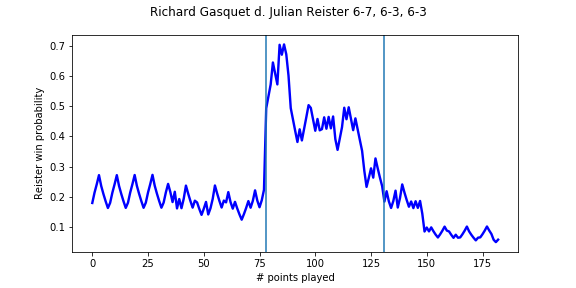
\includegraphics[scale=.7]{gasquet_reister_9_6_all_features}


One drawback of logistic regression is that it cannot distinguish between situations whose score differentials are equivalent. A player serving at (1,0,5,4,3,0) will have approximately the same win probability as one serving at (1,0,1,0,3,0). However, in the first situation from 5-4 40-0, the player serving wins the match if he wins any of the next three points. From the second scenario, the player serving must maintain his lead of 1-0 40-0 throughout the second set, which is less favorable.

Although the first situation is clearly favorable, logistic regression will compute approximately the same probability in both scenarios $\footnote{after fitting coefficients for the equation $P(win) = logit(s_i,s_j,g_i,g_j,{x}_i,{x}_j) = e^{(c_1s_i+c_2s_j+c_3g_i+c_4g_j+c_5x_i+c_6x_j}$, coefficients $ c_1 \approx c_2, c_3 \approx c_4,c_5 \approx c_6$ by symmetry and therefore}$

Another issue is that logistic regression can fail to detect when a higher-ranked player is about to lose in a close match. Below,

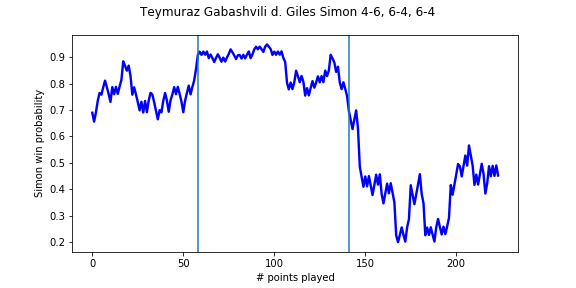
\includegraphics[scale=.7]{simon_gabashvili_9_6_all_features}

\item Random-Forest approach

Brian Burke's win-probability models are among the most well-known in sports. They calculate a team's win probability at any point in the match based on historical data. Nettleton and Lock improved upon this method of binning players together with a random forest approach.

\item See neural nets/mlp paper

\item hierarchical Markov Model: regular and beta model

\item Inferring Serve Probabilities from Elo difference (also try this with Glicko)

In "", Klaassen and Magnus suggest a method to infer serving probabilities from a pre-match win forecast. By imposing a constraint $f_{ij}+f{ji}=1.29$, 



\end{enumerate}
\end{document}